\chapter{Baseline experimental characterization of a high solidity cross-flow
turbine}\label{chap:RVAT-baseline}

As an initial baseline experiment with the turbine test bed, the performance and
near-wake velocity of the high solidity UNH-RVAT were measured. Note that the
results presented here have been published in \cite{,
    Bachant2015-JoT}.

The first task was to assess the rotor's characteristic performance (power and
drag coefficient versus tip speed ratio) curves. Next, a typical operating set
point tip speed ratio was established, at which the near-wake was examined in
detail to gain insight into the mechanisms that improve CFT wake recovery rates
compared with AFTs (allowing closer spacing, \emph{cf.} \cite{Kinzel2012}) or
other axisymmetric turbulent wakes, with the ultimate goal that these mechanisms
can be replicated in simpler models for use in simulations of large turbine
arrays, where resolving actual turbine geometry is prohibitively expensive. The
ability of one such model---an actuator disk inside a Reynolds-Averaged
Navier--Stokes (RANS) simulation---to predict those defining characteristics was
also assessed.

The dominant scales within the turbine's near-wake were evaluated for their
relative importance, loosely following the conceptual framework presented in
Chamorro et al. \cite{Chamorro2012b}, where the turbine was treated as an
``active filter.'' However, by extending this concept it should be cautioned
that this filter could also be nonlinear, i.e., the spectral modifications of
the inflow are dependent on the spectral distribution itself, not a
superposition of effects at each individual scale. It is also expected that a
CFT will introduce even stronger large (turbine) scale variance into the flow,
due to its cyclical forcing from oscillatory blade angles of attack and relative
velocity. The experiments presented here were performed in a towing tank,
providing a very low turbulence intensity inflow (at least as low as the
instrumentation noise floor), which provides an excellent baseline case for
spectral content added to the flow by the turbine, without any modulation of a
turbulent inflow spectra.

Previous detailed experimental studies with CFTs were generally limited in terms
of Reynolds number due to small geometric scale. On the other hand, as expected,
large-scale measurements were typically performed with lower resolution
instrumentation, and with less control of inflow conditions
\cite{Vermeulen1979}. Brochier et al.~\cite{Brochier1986} employed laser-Doppler
velocimetry (LDV) to acquire detailed flow measurements of a small-scale,
quasi-2-D CFT in dynamic stall. Their study was similar in scope to the work
presented here, but was conducted at very low Reynolds number---approximately
two orders of magnitude smaller than the study presented here. More recently,
Tescione et al. \cite{Tescione2014} performed a detailed experimental campaign,
using particle image velocimetry to illuminate vortex structures in the wake,
and how these interact with each other. However, the question still remains as
to why the CFT wake would recover more quickly than that of an AFT. The study
reported here also examined the three-dimensionality of the wake, as turbine
``end effects'' will no doubt affect interaction with the free stream.

To summarize, the goals of this experiment were:
\begin{enumerate}
    \item To identify the essential features of the near-wake of a cross-flow
    turbine.
    
    \item To assess the relative importance of mean and turbulent dynamics on the
    transport of momentum and kinetic energy in the wake.
    
    \item To compare the measured CFT wake to numerical predictions from a
    uniform actuator disk force parameterization implemented inside a RANS
    model, to evaluate its prospects for representing CFTs in array simulations.
\end{enumerate}


\section{Experimental test plan}

All experiments were performed at a tow speed of 1 m/s, resulting in a Reynolds
number based on turbine diameter of $Re_D = U_\infty D /\nu = 1 \times 10^6$, or
an approximate blade chord Reynolds number of $Re_c \approx \lambda U_\infty
c/\nu = 2.7 \times 10^5$ for $\lambda=1.9$, where tip speed ratio $\lambda
\equiv \omega D / (2 U_\infty)$. Note that this Reynolds number is high enough
to be considered operating in a $Re$-independent regime \cite{Bravo2007,
    Bachant2014, Bachant2016-Energies}, which is examined in more detail in
Chapter~\ref{chap:Re-dep}.

The performance of the turbine was measured first by operating at a range of tip
speed ratios, which were held constant during individual tows, and varied from
almost zero to just above that where power becomes negative, i.e., where the
motor has to drive the rotor. From the $C_P$--$\lambda$ curve, the optimal tip
speed ratio $\lambda_0$ was selected for characterizing the wake at one rotor
diameter downstream of the rotor axis. The flow measurements mapped out the
upper half of the turbine wake over 3 m in the spanwise direction, centered
within the 3.66 m tank width, the coordinate system and locations for which are
shown in Figure~\ref{fig:RVAT-baseline-wake-coordinates}.

\begin{figure}
    \centering
    
    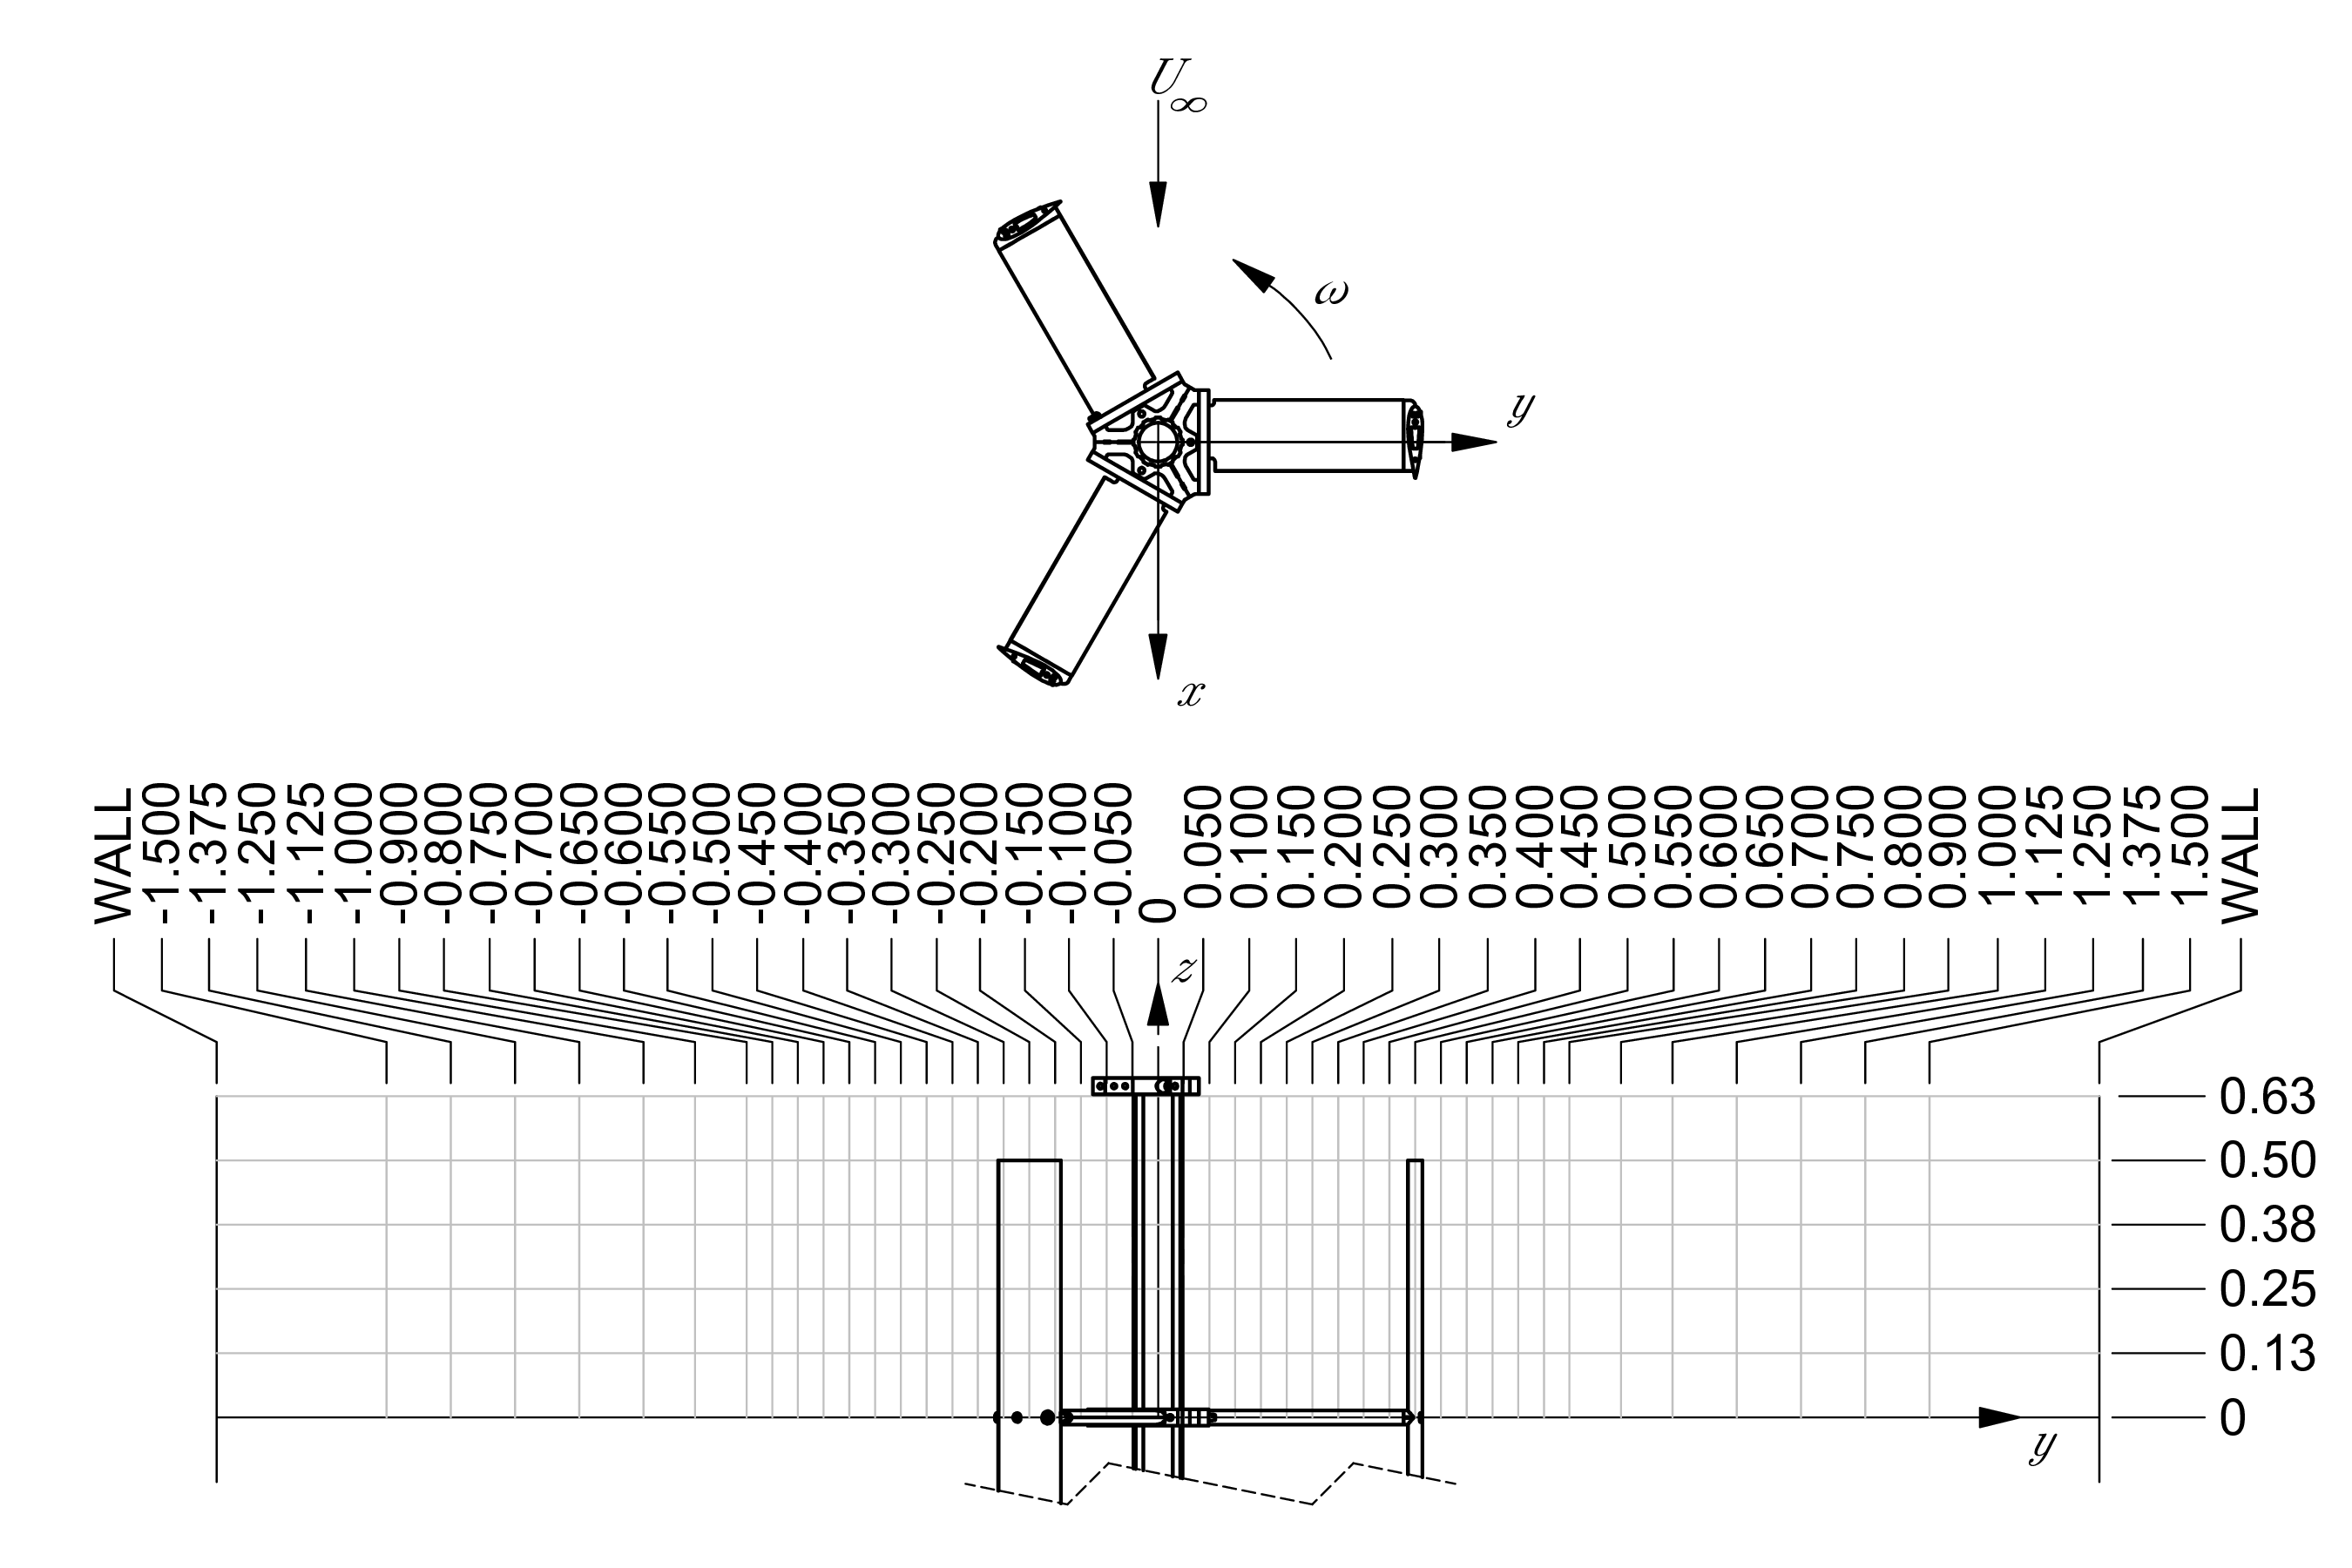
\includegraphics[width=0.99\textwidth]{unh-rvat-coord-sys}
    
    \caption{Wake measurement coordinate system and grid.}
    
    \label{fig:RVAT-baseline-wake-coordinates}
\end{figure}

For the power and drag measurements, the ADV was placed at the quarter height
$z/H = 0.25$, with $z/H=0$ corresponding to the turbine center. A duplicate set
of measurements were also taken for $z/H = 0$ to show how quarter height and
center line measurements differ as a function of tip speed ratio. One additional
transverse wake profile was then acquired at $z/H = 0.25$ for a
lower-than-optimal tip speed ratio to increase the effects of dynamic stall.


\section{Results and discussion}

\subsection{Data processing}

Data from each tow were extracted where the quantities of interest---torque,
drag, and velocity---had reached an approximately stationary mean value. The
time series were then trimmed further such that they correspond to an integer
number of turbine blade passages, to minimize bias from periodicity. Wake data
collection runs included 30 blade passages, which corresponds to approximately
16.5 seconds or 3300 velocity samples at each measuring station. Drag from the
mounting structure, a.k.a. tare drag, was measured by towing with the turbine
removed, and then subtracted from the turbine measurements to provide a better
estimate of the overall drag on the turbine rotor and shaft alone. Similarly,
tare torque was measured by driving the turbine support shaft and bearings in
air and regressing these values linearly with respect to shaft angular velocity.
This tare torque was then added to the measured turbine torque in
post-processing to provide a more accurate estimate for the true hydrodynamic
torque.

As described in Chapter~\ref{chap:exp-setup}, the tank was seeded with 11 $\mu$m
mean diameter hollow glass spheres to achieve adequate beam correlation and
signal-to-noise ratios. No filtering was used on the velocity data, i.e.,
statistics were computed using all raw samples from the measurement interval.
For computing partial derivatives of velocity quantities, a central difference
scheme was employed. For the boundaries of the measurement plane, an
inward-facing second-order scheme was used. The data processing and plotting
code, along with the reduced dataset are available from
\cite{Bachant2014-RVAT-baseline}.


\subsection{Turbine performance}

Performance curves showing the overall power and drag coefficients of the
turbine are shown in Figure~\ref{fig:RVAT-baseline-perf}. The drag coefficient
monotonically increases with increasing tip speed ratio over the entire range
tested, and the power coefficient reaches a maximum of 26\% around a tip speed
ratio $\lambda=1.8$--$1.9$, where the drag coefficient is 0.96. These curves
informed the selection of the optimal tip speed ratio $\lambda_0 = 1.9$ as the
operating point for detailed near-wake characterization. We expect that at this
tip speed ratio the turbine blades will be operating in dynamic stall over a
part of the turbine rotation \cite{Scheurich2011}, reaching maximum angles of
attack of approximately 35 degrees, and that this will be a significant
contributor to the near-wake structure. Note that the maximum power coefficient
could likely be improved with simple geometric modifications, e.g., changing the
blade pitch \cite{Fiedler2009}, but for this study the geometry was meant to be
as simple as possible, therefore the blade pitch was left at zero.

\begin{figure}
    \centering
    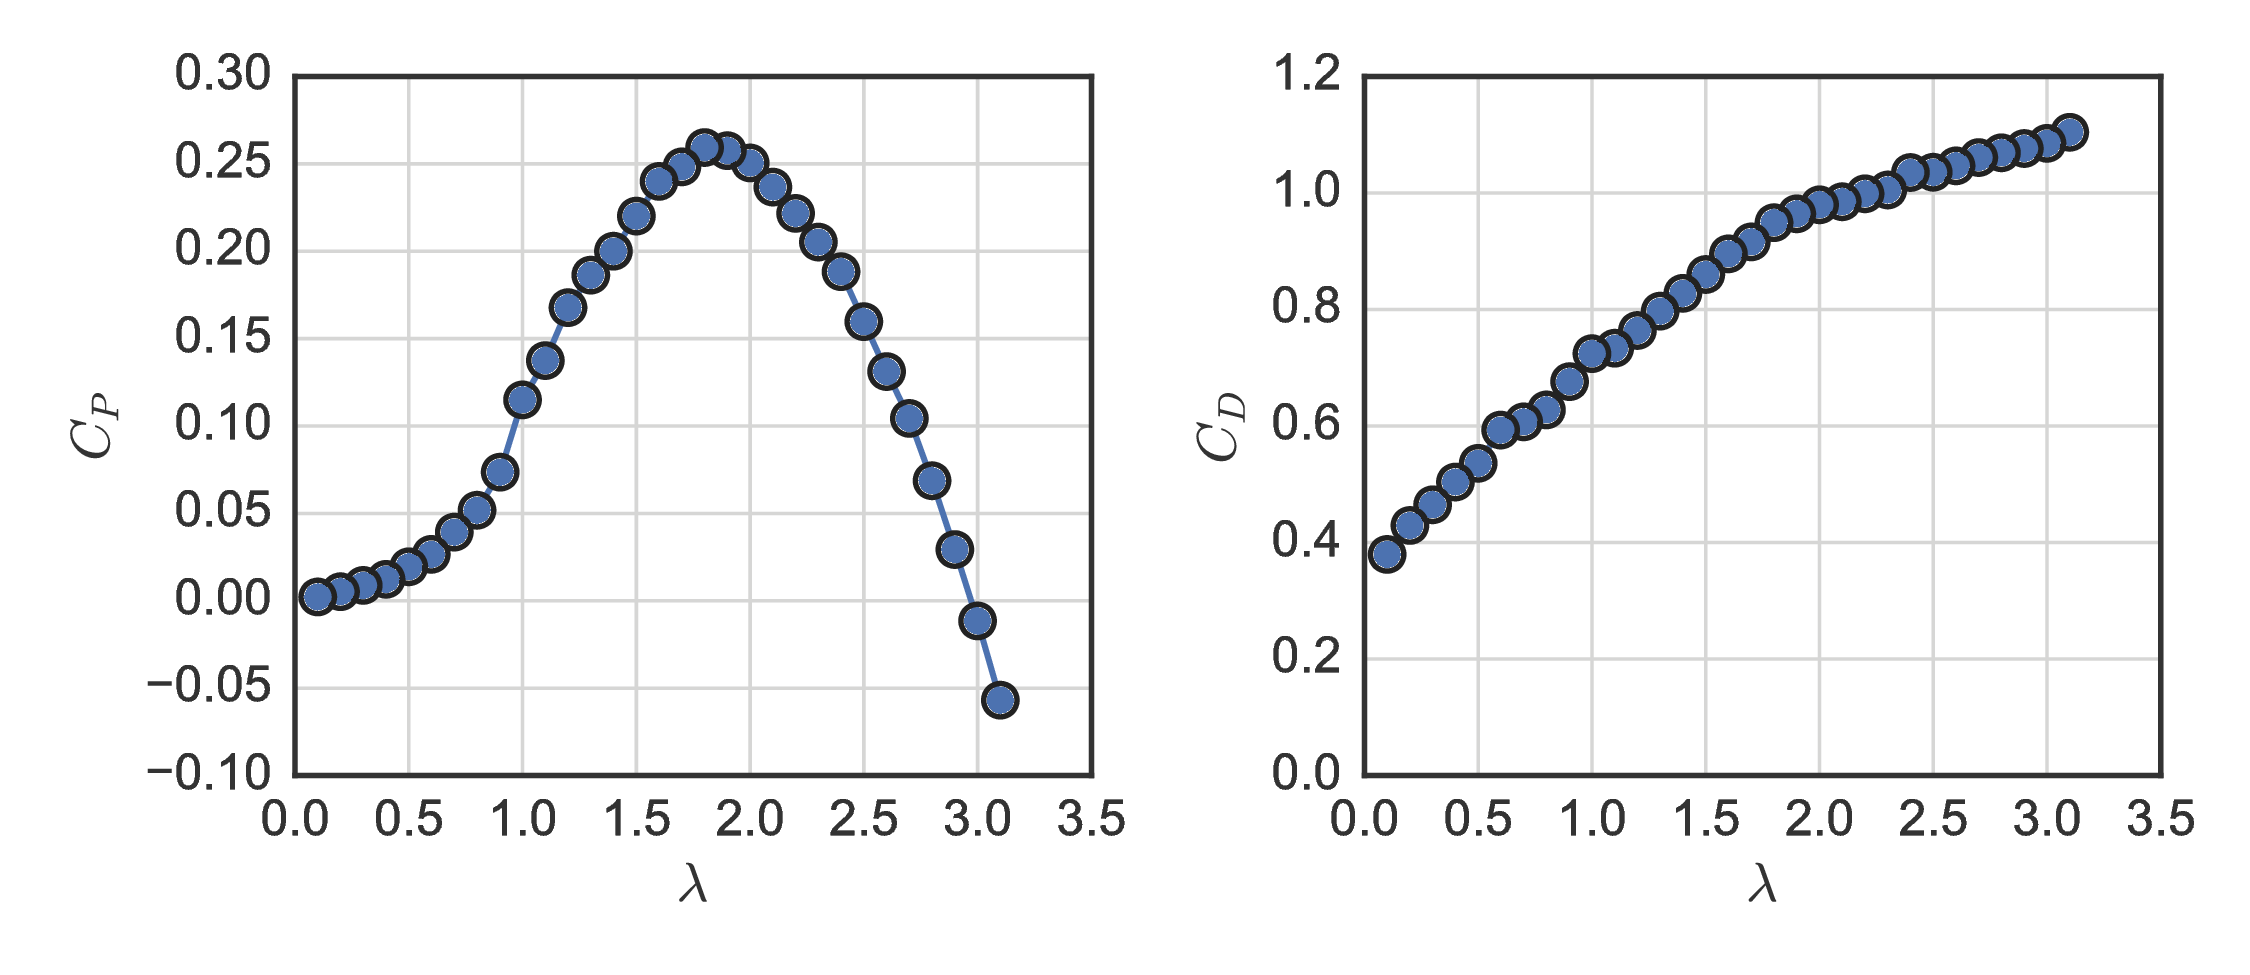
\includegraphics[width=0.9\textwidth]{RVAT-baseline_perf}
    \caption{Mean turbine power (left) and drag (right) coefficients plotted
        versus tip speed ratio.}
    \label{fig:RVAT-baseline-perf}
\end{figure}


\todo[inline]{Add assessment of unsteadiness.}


\subsection{Wake characteristics}

The near-wake of the turbine was described in terms of its mean velocity,
streamwise vorticity, Reynolds stresses, and turbulence kinetic energy. Dominant
time scales were identified and evaluated for their contribution to the turbulent
spectra. Finally, the processes that lead to replenishment of momentum and
energy in the wake were investigated, with the goal of explaining the CFT's
relatively fast wake recovery.


\subsubsection{Momentum and vorticity}

The mean velocity measured in the wake at one turbine diameter downstream is
shown in Figure~\ref{fig:RVAT-baseline-meancontquiv}. The most obvious
characteristics are the asymmetry and three-dimensionality of the flow field.
The peak momentum deficit is shifted towards the right side of the turbine
(looking upstream). We can also see the effects of blade tip vortex shedding,
where flow is moving downward and to the left, creating strong streamwise mean
vorticity near the blade tip at $y/R=-1$, contours for which are shown in 
Figure~\ref{fig:xvorticity}. The asymmetry may explain observations of
counter-rotating turbine pairs helping speed wake recovery \cite{Dabiri2011}.

\begin{figure}
    \centering
    
    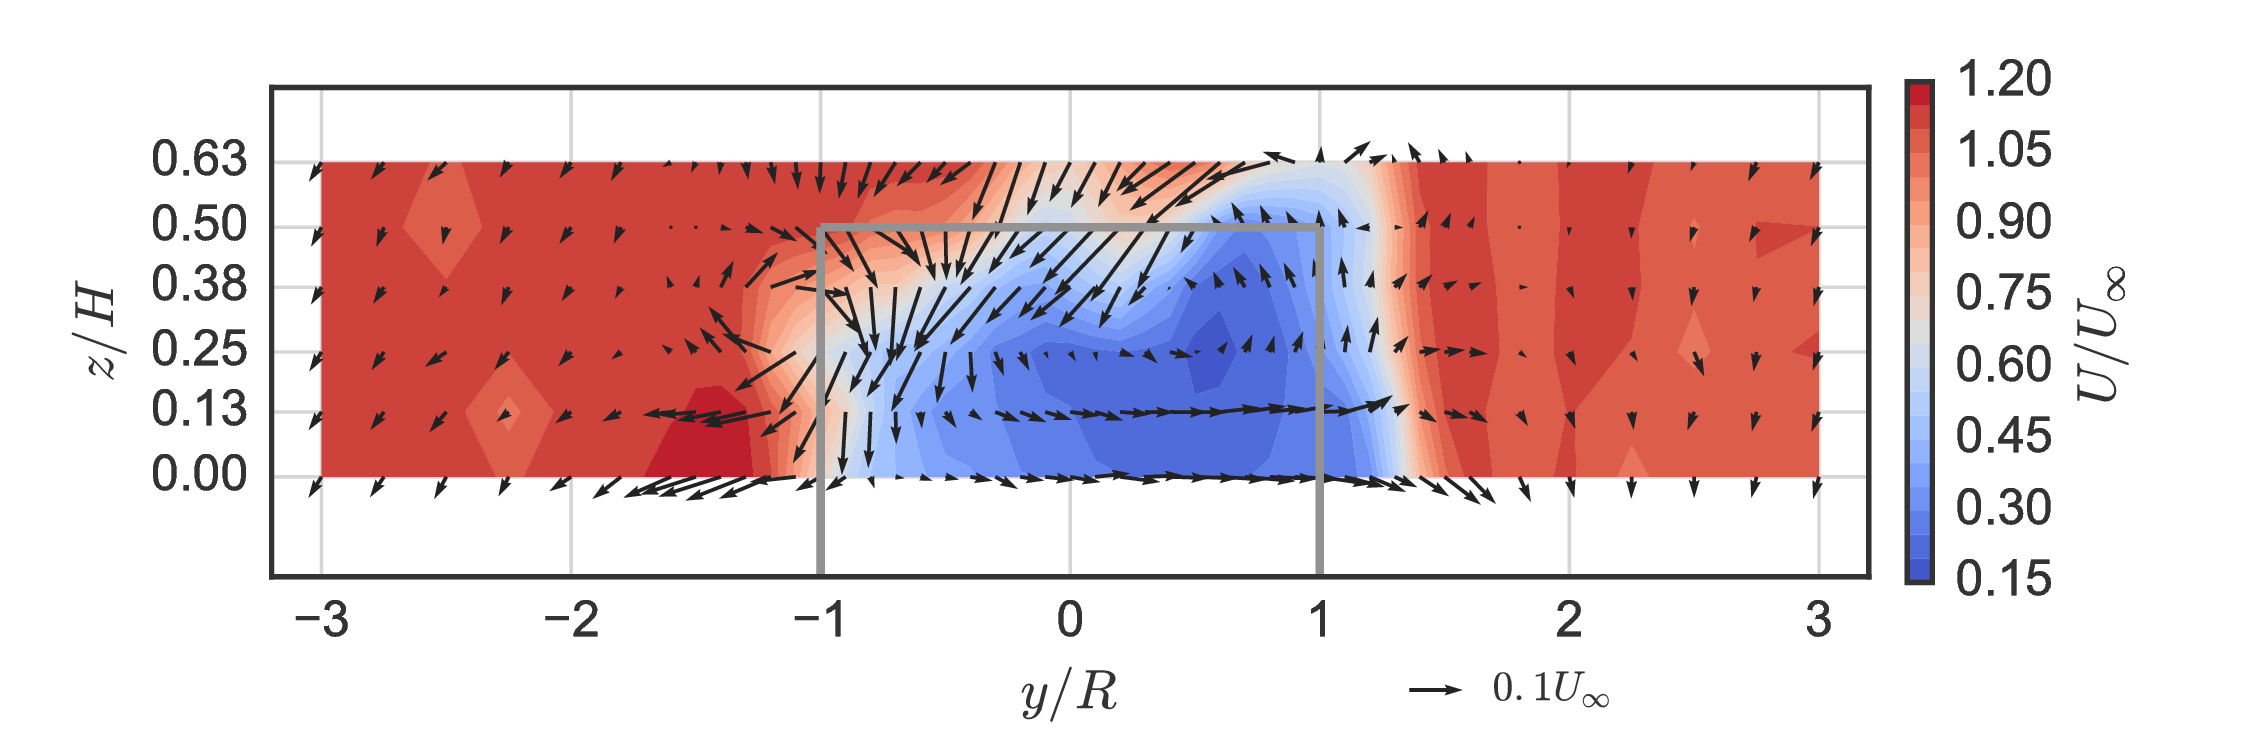
\includegraphics[clip, width=0.9\textwidth]{RVAT-baseline_meancontquiv}
    
    \caption{Mean velocity at $\lambda=1.9$. Vectors are cross-stream and
        vertical velocities; contours are streamwise velocity. View is looking
        upstream, with the turbine frontal area indicated by the solid gray lines.}
    
    \label{fig:RVAT-baseline-meancontquiv}
\end{figure}

The generation of streamwise vorticity with opposing directions highlights once
again the three-dimensionality of the wake of this turbine, and its difference
from an axisymmetric swirling wake such as that of an axial-flow turbine. The
two regions of counter-rotating vorticity act like an asymmetrical doublet,
propelling fluid downward towards the turbine centerline.

Compared with the rotating cylinder wake measurements of Lam~\cite{Lam2009}, we
see a similar asymmetry in the mean streamwise velocity. The wake is less
asymmetrical with respect to the wake centerline for the turbine compared to the
rotating cylinder for the same non-dimensional rotation rate, although some of
these differences may be due to the cylinder experiments' lower Reynolds
numbers. Compared with the end effects of a finite cylinder
wake~\cite{Sumner2004}, we do see generation of a counter-rotating vortex pair,
though for a non-rotating cylinder these are symmetric, which is not the case
for the turbine wake, where the vortex pair seems to be tilted. The turbine's
wake is also similar to a finite cylinder wake in a sense that there is a mean
downward velocity directly behind the wake generator. These similarities and
differences give some perspective regarding the use of cylinders for turbine
simulators in physical model studies of arrays, which was considered
by~\cite{Pierce2013}.

Compared with an axial-flow turbine wake~\cite{Cal2010}, and a rotating actuator
disk model~\cite{Wu2011}, axisymmetric streamwise vorticity or swirl is not
observed here, which is one of the reasons for the wakes' differing dynamics.
This can be explained as a consequence of the conservation of angular momentum,
where the AFT imparts a streamwise rotation along its axis due to torque
generation, where the CFT imparts a torque that is perpendicular to the flow.
The AFT mean swirl only propels fluid away from its axis, while the CFT induces
mean flow into its momentum deficit region, albeit in a asymmetric fashion.

\todo[inline]{Get RVAT-baseline xvorticity fig.}
\begin{figure}
    \centering
    
%    \includegraphics[clip, trim=0 0.3in 0
% 0.3in,width=0.8\textwidth]{RVAT-baseline_xvorticity}

    \caption{Contours of mean streamwise vorticity. Note that this perspective
        is looking upstream and therefore negative values indicate clockwise
        rotation.}
    
    \label{fig:xvorticity}
\end{figure}

Reynolds shear stress contours, shown in Figure~\ref{fig:restress}, quantify the
replenishment of mean momentum by turbulent transport. Regions of high
$\overline{u'v'}$ as well as the observed asymmetry correspond to the regions of
high gradients of streamwise velocity, indicating regions of high turbulence
production.

\todo[inline]{Get RVAT-baseline uvcont and uwcont figs.}
\begin{figure}
    \centering
%    \includegraphics[clip, trim=0 0.3in 0 0.5in, width=0.8\textwidth]{Figures/uvcont}
%    \includegraphics[clip, trim=0 0.3in 0 0.5in, width=0.8\textwidth]{Figures/uwcont}
    \caption{Contours of Reynolds shear stress.}
    \label{fig:restress}
\end{figure}

To quantify the relative importance of mean and turbulent transport processes,
we rearrange the streamwise Reynolds-averaged momentum equation to isolate terms
contributing to its streamwise derivative. Assuming the flow is stationary in
the mean and incompressible, the equation becomes

\begin{equation}
    \begin{split}
        \frac{\p U}{\p x}  =  
        \frac{1}{U} \bigg{[}
        & - V\frac{\p U}{\p y}
        - W\frac{\p U}{\p z} \\
        & -\frac{1}{\rho}\frac{\p P}{\p x} \\
        & - \frac{\p}{\p x} \overline{u'u'}
        - \frac{\p}{\p y} \overline{u'v'}
        - \frac{\p}{\p z} \overline{u'w'} \\
        & + \nu\left(\frac{\p^2 U}{\p x^2}
        + \frac{\p^2 U}{\p y^2}
        + \frac{\p^2 U}{\p z^2} \right)
        \bigg{]}.
    \end{split}
\label{eq:momentum}
\end{equation}

From the experimental measurements, all of the terms on the right hand side were
computed except for the streamwise pressure gradient and the streamwise ($x$)
derivatives of the Reynolds and viscous stresses; the latter two terms are
expected to be small under a thin shear layer assumption. Totals for all these
terms, normalized by $D/U_\infty$ to assess nondimensional mean momentum
recovery per turbine diameter of downstream distance are plotted in
Figure~\ref{fig:mombargraph}. We see that as expected, viscous diffusion is
almost negligible. The two Reynolds stress transport terms are both significant,
but the vertical advection term dominates, and the horizontal advection term
contributes negatively, corresponding to streamlines diverging around the
turbine. The flow essentially behaves like an inviscid three-dimensional,
non-axisymmetric turbulent wake. If we sum all the terms we obtain a total wake
recovery rate at $x/D=1$ of 12\% per turbine diameter, which would be
interesting to compare with an axial-flow turbine in similar conditions.

\todo[inline]{Get RVAT-baseline mombargraph fig.}
\begin{figure}
    \centering
    
%    \includegraphics[clip, trim=0 0.25in 0 0.2in,
% width=0.8\textwidth]{Figures/mombargraph}
    
    \caption{Estimates for the contributions to mean streamwise momentum
        recovery in the streamwise direction, multiplied by two (due to assumed
        symmetry), averaged over the measurement plane, and normalized by the
        average streamwise velocity, freestream velocity, and turbine diameter.}
    
    \label{fig:mombargraph}
\end{figure}


\subsubsection{Dominant time scales}

Spectral densities were computed using a fast Fourier transform (FFT) based
algorithm, with a Hanning window applied to the time series. Spectral values
were averaged over 4 adjacent frequencies to reduce noise and increase
confidence intervals. Figure~\ref{fig:fcont} shows the peak
frequency---normalized by the turbine angular frequency---of the cross-stream
velocity energy spectra at each measurement point. We can see how unsteadiness
in the flow is induced primarily at the blade passage frequency, or three times
$f_\mathrm{turbine}$. Note that some higher peak frequencies can also be seen in
this plot, out in regions of low turbulence intensity. This is due to both the
noise floor of the ADV and the wakes of the guy wire supports.

Spectral concentration $\Psi$ is quantified by normalizing the peak value of the
spectral density by the total variance of the signal multiplied by the
spectrum's Fourier frequency interval $\Delta f$, i.e.,
\begin{equation}
    \Psi \equiv \frac{S_{\max} \Delta f}{\sigma^2},
    \label{eq-spec_cont}
\end{equation}
where $\Delta f \equiv 1/(N \Delta t)$, $N$ is the total number of samples, and
$\Delta t$ is the sampling interval. For a pure harmonic $\Psi = 1$, indicating
all variance contained within a single frequency. This metric provides further
characterization of the turbulence in terms of its range of scales, rather than
the overall variance or turbulence intensity.

A plot of this concentration is also shown in Figure~\ref{fig:fcont}, where it
is evident that energy is more concentrated towards the side of the  turbine
where the blades move upstream, likely seeing lower angles of attack, and
therefore boundary layer separation occurring further towards the trailing edge
of the blade. This concentration is indicative of more coherent motion, or
extraction of energy/momentum from the flow without intense separation, whereas
on the opposite side of the turbine, turbulence generated by the dynamic stall
process is increasing the diffusion of shed vorticity. This effect can be
further illustrated looking at sample spectra for turbine torque coefficient and
cross-stream velocity components at two points on opposite sides of the turbine,
shown in Figure~\ref{fig:multispec}, where the cross-stream velocity at the side
of the turbine inducing massive separation shows a smaller peak in its spectrum
at the blade passage frequency.

\todo[inline]{Get RVAT-baseline fpeak\_v and fstrength\_v figs.}
\begin{figure}[h]
    \centering
    
%    \includegraphics[clip, trim=0 0.3in 0 0.5in,
% width=0.8\textwidth]{RVAT-baseline_fpeak_v}
%    \includegraphics[clip, trim=0 0.3in 0 0.3in,
% width=0.8\textwidth]{RVAT-baseline_fstrength_v}

    \caption{Cross-stream velocity energy spectra peak frequency normalized by
        turbine angular frequency (top) and spectral concentration (bottom). Note
        that white regions have values higher than the maximum value of the color
        bar, caused by both noise and wakes of the guy wire supports.}
    
    \label{fig:fcont}
\end{figure}

\todo[inline]{Get RVAT-baseline multispec fig.}
\begin{figure}
    \centering

%    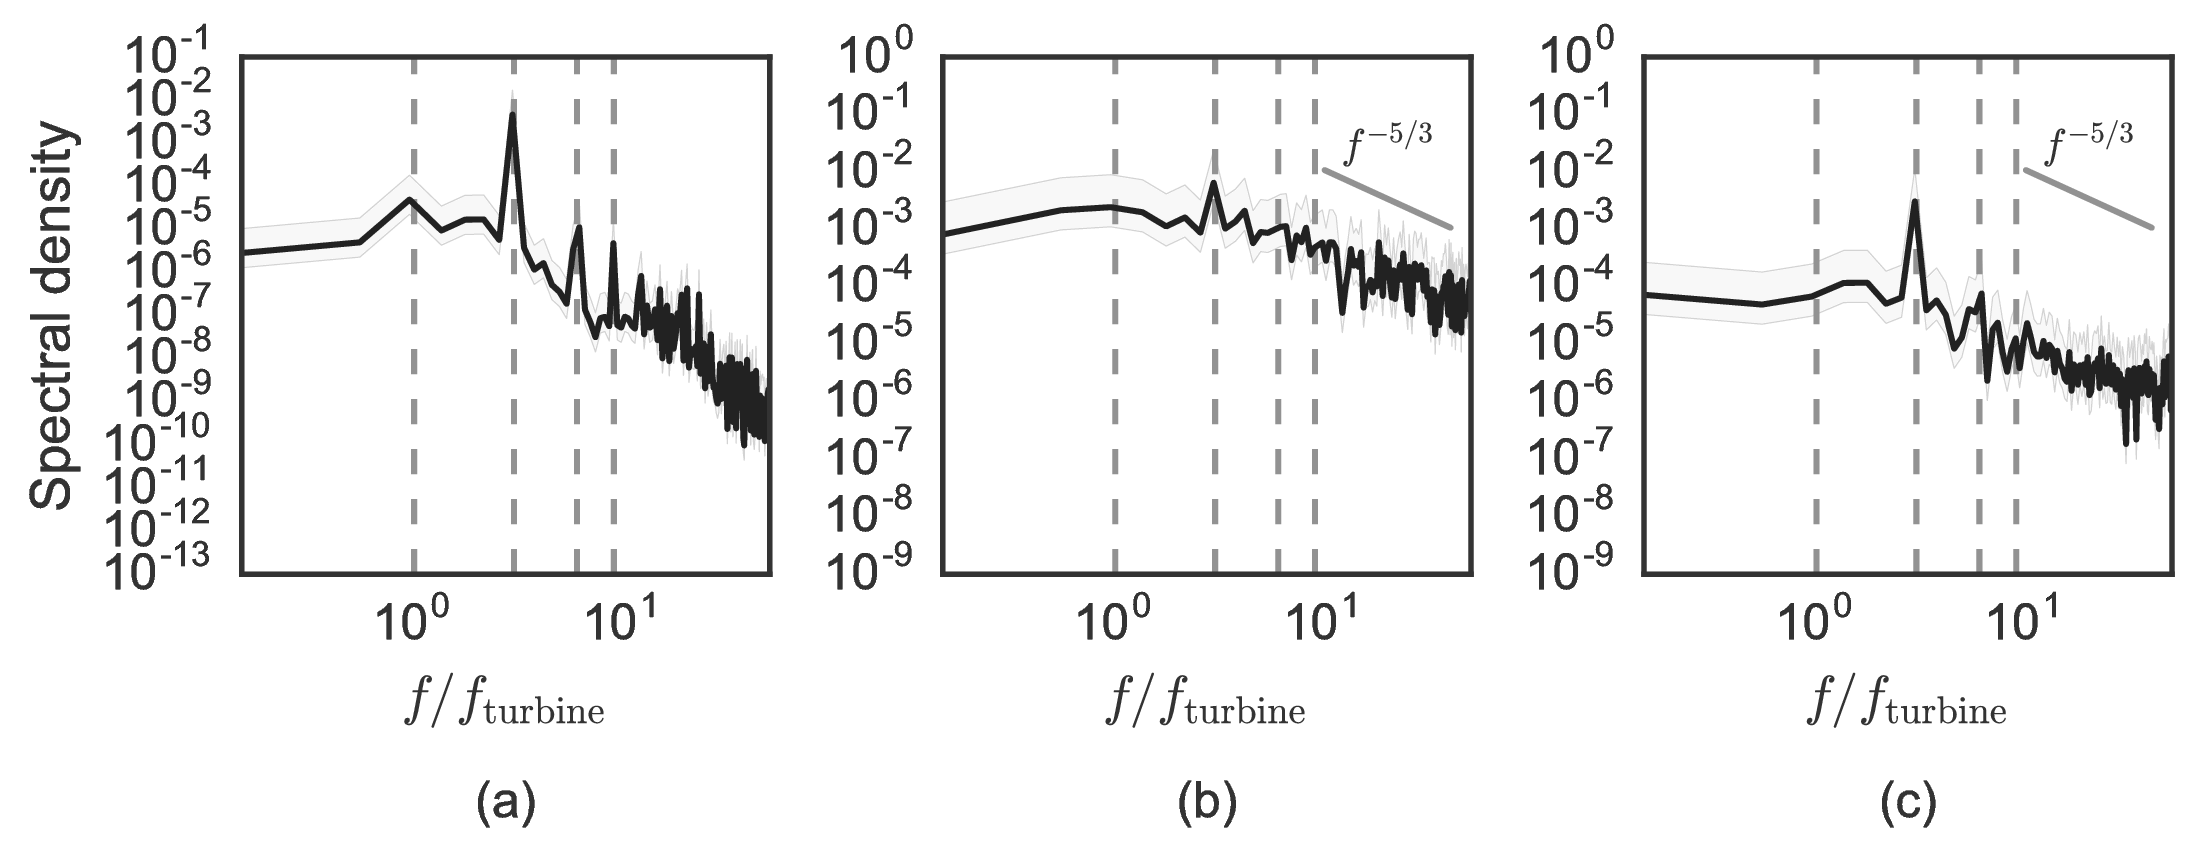
\includegraphics[width=0.98\textwidth]{RVAT-baseline_multispec}

    \caption{Spectral density for (a) torque coefficient, (b) cross-stream
        velocity at $y/R = -1$; $z/H = 0.25$, and (c) cross-stream velocity at $y/R
        = 1.5$; $z/H = 0.25$. Dashed vertical lines indicate $[1, 3, 6, 9]$ times
        the turbine rotational frequency and the shaded gray region indicates the
        95\% confidence interval for a $\chi^2$ variable with 8 degrees of
        freedom---twice the number of frequencies over which spectral values were
        averaged to reduce noise.}
    
    \label{fig:multispec}
\end{figure}


\subsubsection{Kinetic energy}

Contours of turbulence kinetic energy are shown in Figure~\ref{fig:kcont}. The
turbulence kinetic energy is concentrated near the top and left side of the
turbine, as a result of the blade tip and dynamic stall vortex shedding,
respectively. The lower turbulence kinetic energy on the $+y$ side of the
turbine corresponds with the more concentrated spectral energy of velocity
unsteadiness in this area. This can be interpreted as the lift-induced vorticity
being shed with less separation compared to the $-y$ side of the turbine, where
turbulence is being generated and redistributing energy across a larger
bandwidth. This brings up one potential improvement to actuator line models:
Modulating turbulence fields at the occurrence of dynamic stall.

\todo[inline]{Get RVAT-baseline kcont fig.}
\begin{figure}
    \centering

%    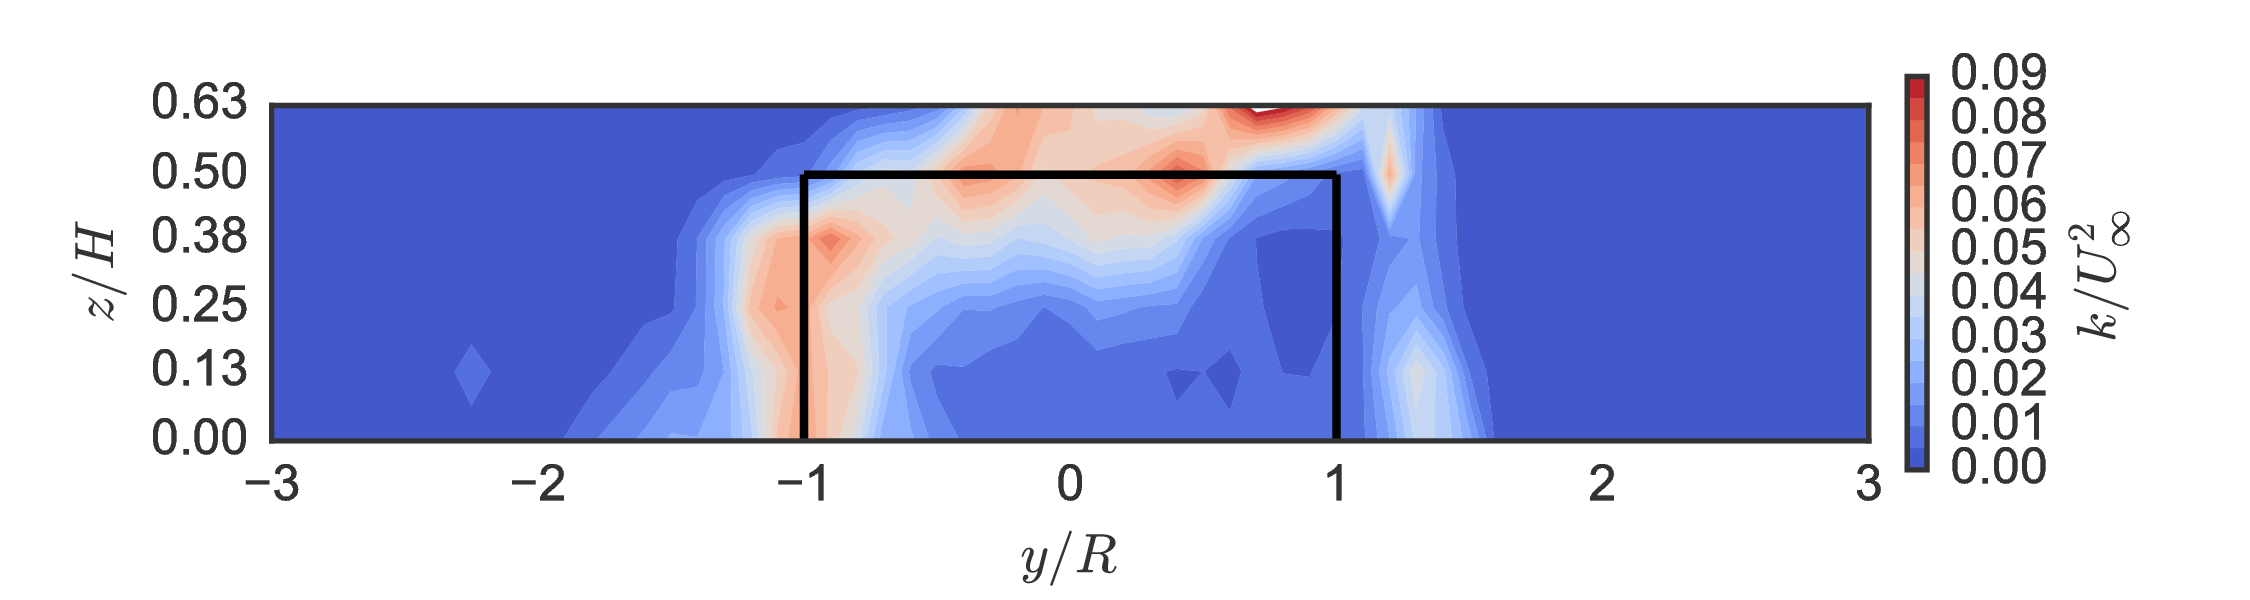
\includegraphics[clip, trim=0 0.25in 0 0.3in,
% width=0.8\textwidth]{RVAT-baseline_kcont}

    \caption{Contours of turbulence kinetic energy, normalized by the mean
        freestream kinetic energy. Turbine frontal area is indicated by solid black
        lines.}
    
    \label{fig:kcont}
\end{figure}

Like the analysis of the mean streamwise momentum, the mechanisms which play the
most important role in mean kinetic energy recovery as the wake evolves in the
streamwise direction are now examined. The transport equation for the kinetic
energy $K$ associated with the mean flow \cite{TennekesAndLumley}, rearranged to
isolate the streamwise recovery can be written as
\begin{equation}
    \begin{split}
        \frac{\p K}{\p x}
        =
        \frac{1}{U}
        \bigg{[}
        & - \underbrace{V \frac{\p K}{\p y}}_{y\text{-adv.}}
        - \underbrace{W \frac{\p K}{\p z}}_{z\text{-adv.}}
        % Pressure work:
        - \frac{1}{\rho}\frac{\p}{\p x_j} P U_i \delta_{ij}
        % Work by viscous forces
        + \frac{\p}{\p x_j} 2 \nu U_i S_{ij}
        % Turbulent transport of K
        - \underbrace{
            \frac{1}{2}\frac{\p}{\p x_j} \overline{u_i' u_j'} U_i
        }_{\text{Turb. trans.}} \\
        % Production of k
        & + 
        \underbrace{
            \overline{u_i' u_j'} \frac{\p U_i}{\p x_j}
        }_{k\text{-prod.}}
        - 
        \underbrace{
            2 \nu S_{ij}S_{ij}
        }_{\text{Mean diss.}}
        \bigg{]}.
    \label{eq-K_full}
    \end{split}
\end{equation}
The terms of interest are labeled---advection in the cross-stream and vertical
directions, energy transport by turbulent fluctuations, production of turbulence
kinetic energy $k$ through mean shear, and the dissipation due to mean viscous
shear forces. For the tensor terms, streamwise derivatives were ommitted, since
the measurements were limited to a single streamwise distance.
Table~\ref{tab:RVAT-baseline-eqs} lists all components kept for the computation
of each transport term.

\begin{table}
    \centering
    \begin{tabular}{c|c}
        Term in Eq.~\ref{eq-K_full} & Implementation \\ 
        \hline  
        $y$-adv. & $-\frac{V}{U}\frac{\p K}{\p y}$ \\ 
        $z$-adv.  & $-\frac{W}{U}\frac{\p K}{\p z}$ \\ 
        Turb. trans. ($y$) & $-\frac{1}{2U} \big{[} \frac{\p }{\p y}\overline{u'v'}U 
        + \frac{\p }{\p y}\overline{v'v'}V + \frac{\p }{\p y}\overline{w'v'}W \big{]} $\\ 
        Turb. trans. ($z$)  & $-\frac{1}{2U} \big{[} \frac{\p }{\p z}\overline{u'w'}U 
        + \frac{\p }{\p z}\overline{v'w'}V + \frac{\p }{\p z}\overline{w'w'}W \big{]} $\\ 
        $k$-prod.  & $\frac{1}{U} \big{[} \overline{u'v'}\frac{\p U}{\p y}
        + \overline{v'v'}\frac{\p V}{\p y} 
        + \overline{w'v'}\frac{\p W}{\p y} $ \\
        & $ + \overline{u'w'}\frac{\p U}{\p z}
        + \overline{v'w'}\frac{\p V}{\p z}
        + \overline{w'w'}\frac{\p W}{\p z}
        \big{]} $ \\ 
        Mean diss.   & $ - \frac{2 \nu}{U} \big{[}
        \big{(} \frac{\p U}{\p y} \big{)}^2
        + \big{(} \frac{\p U}{\p z} \big{)}^2
        + \big{(} \frac{\p V}{\p y} \big{)}^2 $ \\
        & $
        + \big{(} \frac{\p V}{\p z} \big{)}^2
        + \big{(} \frac{\p W}{\p y} \big{)}^2
        + \big{(} \frac{\p W}{\p z} \big{)}^2
        \big{]} $ \\ 
    \end{tabular} 
    \caption{Terms used to compute contributions to mean kinetic energy recovery.}
    \label{tab:RVAT-baseline-eqs}
\end{table}

Figure~\ref{fig:RVAT-baseline-Kturbtrans} shows estimates of mean kinetic energy
transport by turbulent fluctuations. The structure of this plot indicates that
the turbulent fluctuations transport mean kinetic energy inward towards regions
of lower mean momentum and lower mean kinetic energy. The signs of the terms
plotted here can be understood from Figures 6 and 4. Note that despite lower
turbulence kinetic energy on the $+y$ side of the turbine, magnitudes of the
turbulent transport are similar on both.


\begin{figure}
    \centering
    
%    \includegraphics[clip, trim=0 0.25in 0 0.3in, width=0.8\textwidth]{Figures/Kturbtrans}

    \caption{Contours of estimated mean kinetic energy transport by turbulent
        fluctuations, where streamwise derivatives are omitted. Turbine frontal area
        is indicated by solid black lines.}
    
    \label{fig:RVAT-baseline-Kturbtrans}
\end{figure}

Contributions to mean kinetic energy recovery from various mechanisms were
averaged over the  measurement plane using the trapezoidal rule.
Figure~\ref{fig:RVAT-baseline-Kbargraph} shows the normalized sum of each
quantity to show their relative size. As with the momentum, the cross-stream
mean advection contributes negatively since the flow is accelerating around the
turbine due to its pressure disturbance, where streamlines diverge.

Viscous dissipation due to mean shear is essentially negligible compared to
the other terms, which is to be expected in a high Reynolds number shear flow a 
short distance downstream of the shear flow (wake) generator (CFT).

Production of turbulence kinetic energy acts to reduce mean kinetic energy, as
expected for the mean kinetic energy equation. The turbulent transport terms,
separated by the direction of their divergence, i.e., ``$y$-turb.'' is a sum of
all terms with $\p / \p y$ in them and ``$z$-turb.'' is a sum of all terms with
$\p / \p z$ in them, are about the same order of magnitude, both roughly an
order of magnitude smaller than the vertical advection term, which is the
largest. It should be re-stated that the terms in
Figure~\ref{fig:RVAT-baseline-Kbargraph} were evaluated in the near wake, in a
measurement plane at $x/D=1$ shown in
Figure~\ref{fig:RVAT-baseline-wake-coordinates}.

Compared to the observations of Kinzel et al. \cite{Kinzel2012}, where the
turbulent transport terms were found to be not large enough to replenish turbine
power output, it can be seen here that it is most likely vertical advection that
plays the most important role in enhancing the wake recovery, not the turbulence
quantities. This is likely a consequence of the unique vorticity generation and
interaction from lift production, (dynamic) stall vortices, and blade end
effects.

\todo[inline]{Get RVAT-baseline Kbargraph fig.}
\begin{figure}
    \centering
    
%    \includegraphics[clip, trim=0 0.25in 0 0.2in, width=0.8\textwidth]{Figures/Kbargraph}

    \caption{Estimates for the contributions to mean kinetic energy recovery in
        the streamwise direction, multiplied by two (due to assumed symmetry),
        averaged over the measurement plane, and normalized by the average
        streamwise advection velocity, freestream kinetic energy, and turbine
        diameter.}
    
    \label{fig:RVAT-baseline-Kbargraph}
\end{figure}


\todo[inline]{Tweak content from FEDSM paper.}
%%% Below from FEDSM paper


\subsection{Effects of tip speed ratio}

From our measurements we can observe how mean velocities at two fixed points
downstream of the turbine axis vary with tip speed ratio. These velocity
components are shown in Fig.~\ref{fig:meanuvstsr}. Mean streamwise velocity
deficit at at $z/H = 0$ increases with tip speed ratio, which is expected in
light of the drag measurements. However, mean velocity deficit at the quarter
height is highest at tip speed ratios corresponding to high power coefficient,
but decreases at higher values of $\lambda$. Mean vertical velocity at the
turbine center remains relatively constant across the entire operating envelope,
implying the wake is approximately symmetric about $z/H = 0$. However, mean
vertical velocity at the quarter height shows a markedly higher downward
component at higher $\lambda$, corresponding to the similar aforementioned trend
of decreasing streamwise velocity deficit at that location. Since drag
coefficient continuously increases with $\lambda$, we are led to believe the
turbine is becoming more like a solid cylinder, letting less flow through,
therefore more fluid must flow over the top. Asymmetry about $y/R=0$ is seen in
the mean cross-stream velocity at values of $\lambda$ away from those of highest
power output, with a mean component in the positive $y$-direction.

% Mean velocity vs tsr
\begin{figure}[t]
%    \includegraphics[scale=0.42]{Figures/meanuvstsr.pdf}

    \caption{Normalized centerline mean velocity components at $x/D=1$ versus
        tip speed ratio. Filled markers indicate measurements at $z/H=0$, while open
        markers indicate those at $z/H=0.25$.}

    \label{fig:meanuvstsr} 
\end{figure}

Next we want to look more closely at the effects of lowering $\lambda$, thereby
increasing maximum blade angle of attack and inducing increased stalling
behavior. Quarter height streamwise mean velocity profiles for the two tip speed
ratios of interest are shown in Fig.~\ref{fig:meanu_2tsrs}. Some similarities
can be identified with the study by Brochier et al., namely the assymetry of the
wake and how its shape changes on the side of the turbine where the blade faces
into the flow---positive $y$ for our experiments and negative for theirs
\cite{brochier86}.

Regarding turbulence intensity in the wake, we can make similar comparisons. The
data in Brochier et al. shows two peaks on opposite sides of the turbine axis,
with the lower tip speed ratio case having a relatively higher peak on one side
\cite{brochier86}, which should correspond to negative $y$ values in our case.
This is somewhat in agreement with our results, though the value at the origin
for our case is relatively higher, which may be due to the larger shaft wake.
However, when we compare our two profiles, we notice for the lower value of
$\lambda$ there is higher average turbulence intensity throughout the center
region. This appears to be caused by more intense blade stall, beginning earlier
along the blade path, i.e. at higher positive values of $y$. This effect is seen
in all three components of turbulence intensity, agreeing with our earlier
observations of local isotropy.

% Check above!
Fig.~\ref{fig:meanw_2tsrs} shows mean vertical velocity profiles for the two tip
speed ratios of interest. The large gradient appearing at negative values of
$y$, suspected to be the result of blade tip vortices, remains a approximately
the same location. However, the peak seen at $y/R = 1.2$ is decreased for the
lower tip speed ratio case.

Fig.~\ref{fig:meanv_2tsrs} shows profiles of mean cross-stream velocity. Unlike
the streamwise and vertical profiles, these show relatively large differences at
our two tip speed ratios of interest, indicating significant fluid motion---on
the order of 10\% of the free stream velocity---to the left on the left edge of
the rotor at $\lambda=1.9$ and to the right at the right edge of the rotor at
$\lambda = 1.4$.

Fig.~\ref{fig:uv_2tsrs} shows profiles of $\overline{u'v'}$ Reynolds stress.
Similar to the profiles of $\sigma_u$ in Fig.~\ref{fig:stdu_2tsrs}, we see a
rightward shift of the left peak from what we infer is earlier blade stall,
while the right hand peaks are almost identical. In Fig.~\ref{fig:vw_2tsrs}, we
see that profiles of $\overline{v'w'}$ Reynolds stress contain peaks once again
on the left side of the turbine, but the correlations are opposite for the two
tip speed ratios.

% Mean streamwise velocity profiles for 2 tsrs
\begin{figure}[t]
%    \includegraphics[scale=0.42]{Figures/meanu_2tsrs.pdf}

    \caption{Streamwise mean velocity profiles for $\lambda = 1.9$ and
        $\lambda=1.4$ at $x/D=1$ and $z/H = 0.25$.}

    \label{fig:meanu_2tsrs} 
\end{figure}

% Mean vertical velocity profiles for 2 tsrs
\begin{figure}[t]
%    \includegraphics[scale=0.42]{Figures/meanw_2tsrs.pdf}

    \caption{Mean vertical velocity profiles for $\lambda = 1.9$ and
        $\lambda=1.4$ at $x/D=1$ and $z/H = 0.25$.}

    \label{fig:meanw_2tsrs} 
\end{figure}

% Mean cross-stream velocity profiles at 2 tsrs
\begin{figure}[t]
%    \includegraphics[scale=0.42]{Figures/meanv_2tsrs.pdf}

    \caption{Mean cross-stream velocity profiles for $\lambda = 1.9$ and
        $\lambda=1.4$ at $x/D=1$ and $z/H = 0.25$.}

    \label{fig:meanv_2tsrs} 
\end{figure}

% Std u profiles at 2 tsrs
\begin{figure}[t]
%    \includegraphics[scale=0.42]{Figures/stdu_2tsrs.pdf}

    \caption{Streamwise turbulence intensity for $\lambda = 1.9$ and
        $\lambda=1.4$ at $x/D=1$ and $z/H = 0.25$.}

    \label{fig:stdu_2tsrs} 
\end{figure}

% uv Re stress profiles at 2 tsrs
\begin{figure}[t]
%    \includegraphics[scale=0.42]{Figures/uv_2tsrs.pdf}

    \caption{$\overline{u'v'}$ Reynolds stress profiles for $\lambda = 1.9$ and
        $\lambda=1.4$ at $x/D=1$ and $z/H = 0.25$.}

    \label{fig:uv_2tsrs} 
\end{figure}

% vw Re stress profiles at 2 tsrs
\begin{figure}[t]
%    \includegraphics[scale=0.42]{Figures/vw_2tsrs.pdf}

    \caption{$\overline{v'w'}$ Reynolds stress profiles for $\lambda = 1.9$ and
        $\lambda=1.4$ at $x/D=1$ and $z/H = 0.25$.}

    \label{fig:vw_2tsrs} 
\end{figure}


%%% End FEDSM content


\subsection{Comparison with an actuator disk}

The actuator disk model, commonly used in modern large-eddy simulations of wind
farms \cite{Stevens2014}, parameterizes turbine forcing on the flow field as a
steady streamwise force applied over the frontal area of the turbine. The model
is attractive due to its relatively simple implementation; it does not require
the meshing of actual turbine geometry, making it computationally feasible to
simulate large turbine arrays. For example, the turbine array being installed by
ORPC in Cobscook Bay, Maine was laid out with a RANS actuator disk model, where
cross-flow turbines were represented inside the mesh over three cells
\cite{Nelson2013}. Furthermore, the actuator disk force coefficients are not
time dependent, allowing for simulation of, e.g., tidal cycles without the need
for small time steps to resolve unsteady turbine forcing.

Here the experimental measurements are compared and contrasted with the
near-wake of an actuator disk model, to illustrate how this model would
represent a cross-flow turbine in an array simulation. Since one of the
potential benefits of cross-flow turbines is to be able to be spaced more
closely in an array installation, the near-wake dynamics will be more important
than those of an axial-flow turbine.

For axial-flow turbines, the actuator disk model can be enhanced with a rotating
axial velocity component, which gives better results than a simple volume force
\cite{Wu2011}, but to our knowledge this technique has not been applied
(adapted) to cross-flow turbines. Nevertheless, in the present study the
ability of a simple streamwise force distributed over a cylindrical volume to
mimic the near-wake of a cross-flow turbine was evaluated. As described in
previous sections, the asymmetry of the turbine's wake indicates that a uniform
streamwise force from the actuator disk will likely not capture the wake
accurately.

\todo[inline]{Check OpenFOAM version used for AD simulation.}

The open source CFD package \textit{OpenFOAM} was used to solve the RANS
equations with the turbine represented by an actuator disk, which is
implemented as a force or sink in the momentum equation, applied over a selected
volume of cells in the mesh.

The cross-section of the domain is the same as that of the tow tank used for the
experimental measurements. The actuator disk is technically not a disk, but a 1
m diameter by 1 m tall cylinder, mimicking the turbine swept area. The domain
extends 2 m upstream and 8 m downstream.  The background mesh consists of 96,
64, and 48 points in the $x$, $y$, and $z$ directions, respectively. The cells
in the volume enclosed by the actuator disk region are refined by a factor of
two, giving a total of  approximately $3 \times 10^5$ hexahedral cells. A
snapshot of the mesh is shown in Figure~\ref{fig:AD-mesh}. Boundary conditions
are set to approximate the tow tank environment, i.e., the velocity at the
bottom and walls is set to the free stream value. The free surface was not
modeled---the domain had a rigid lid with a slip velocity boundary condition---a
reasonable approximation for low Froude numbers. Inputs to \textit{OpenFOAM}'s
\texttt{actuationDiskSource} are given in Table~\ref{tab:AS}, and the case files
for this simulation are available from \cite{Bachant2014-OF-AS-case-files}.

\begin{figure}
    \centering

    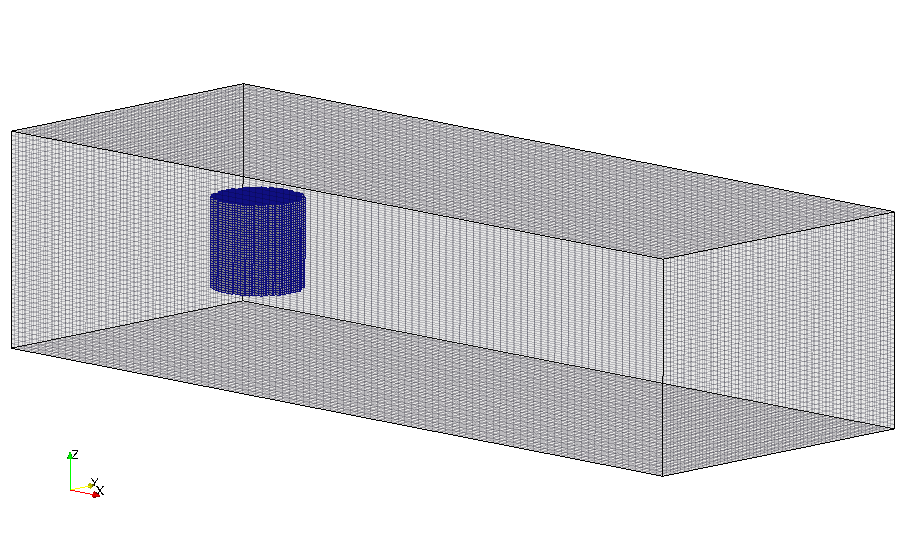
\includegraphics[width=0.9\textwidth]{AD_mesh}

    \caption{Snapshot of the computational mesh for the actuator disk RANS
        simulation.}
    
    \label{fig:AD-mesh}
\end{figure}

\begin{table}
    \begin{center}
        \begin{tabular}{r|l}
            \texttt{Cp} & \texttt{0.26} \\ 
            \texttt{Ct} & \texttt{0.96} \\ 
            \texttt{diskArea} & \texttt{1.0} \\ 
            \texttt{upstreamPoint} & \texttt{(-1.0 0 0)} \\ 
        \end{tabular} 
        \caption{Input parameters for the actuator surface using \textit{OpenFOAM}'s
            \texttt{actuationDiskSource}.}
    \label{tab:AS}
    \end{center}
\end{table}

The turbulence is modeled with a standard $k$-$\epsilon$ closure, with
relatively low levels of inlet turbulence kinetic energy and dissipation, $2
\times 10^{-4}$ and $3 \times 10^{-5}$, respectively. These low free stream
values were chosen to approximate the tow tank ambient conditions.

Results for the mean velocity field are presented in
Figure~\ref{fig:AD-contours}, in a manner similar to that of
Figure~\ref{fig:RVAT-baseline-meancontquiv}, for comparison. The vertical mean
flow, which was determined to be an important driver of near-wake dynamics in
the experiments, is absent. In fact, it contributes negatively to streamwise
wake recovery. This means that all momentum and energy transport back into the
deficit in the wake created by the turbine will need to be facilitated by
turbulent transport (and viscous diffusion, to a much lesser degree). Note also
how acceleration due to blockage is much lower compared to the experiments
despite matching the overall drag coefficient.

Figure~\ref{fig:AD-streamwise} shows the downstream evolution of the centerline
streamwise velocity, and the terms that contribute to its streamwise derivative
averaged over various constant-$x$ planes. Note how very close to the turbine,
the streamwise pressure gradient is contributing significantly to the increase
in $U$, despite the fact that the turbine creates a positive pressure gradient
along the centerline. The large pressure-driven increase in streamwise velocity
makes sense considering the fact that the values are averaged over the entire
cross-section of the domain, which includes a large area of flow acceleration
around the turbine, where the streamwise pressure gradient is negative. Just
after the turbine, $-\p P / \p x$ drops off very quickly and then acts to
decrease streamwise momentum slightly as the static pressure recovers moving
downstream.

We can see that the streamwise momentum recovers very slowly, only starting to
recover around $x=7D$, which can be mostly attributed to the low inflow
turbulence levels, chosen to mimic the tow tank environment. This can be further
understood by looking at the transport terms plotted on the right in
Figure~\ref{fig:AD-streamwise}, where we see all terms are quite small when
compared with the experimental results from the turbine. Rather than the
advection terms, which contribute negatively, the turbulent transport---here
modeled using the $k$--$\epsilon$ eddy viscosity $\nu_t$---is driving the
streamwise evolution, despite being very small. One way to increase the wake
recovery in such a model is to have the actuator disk ``inject'' turbulence
quantities to increase the eddy viscosity \cite{James2011, Nelson2013}. However,
this will likely still not be sufficient to predict evolution and interaction in
closely-spaced arrays of CFTs, since neither the significant vertical mean 
velocities in the CFT wake, nor any coherent vortical structures 
due to blade, shaft, or strut forces are captured by the actuator disk model.

It could be argued that the actuator disk model should not be judged this way as
it is well known that it is a poor predictor of near-wake characteristics,
however, these models are common in engineering practice when calculating
performance of turbine arrays, as previously mentioned. The experiments reported
here have shown that the use of these models would likely be a source of large
uncertainty if applied to cross-flow turbine installations.

\begin{figure}
    \centering
    
    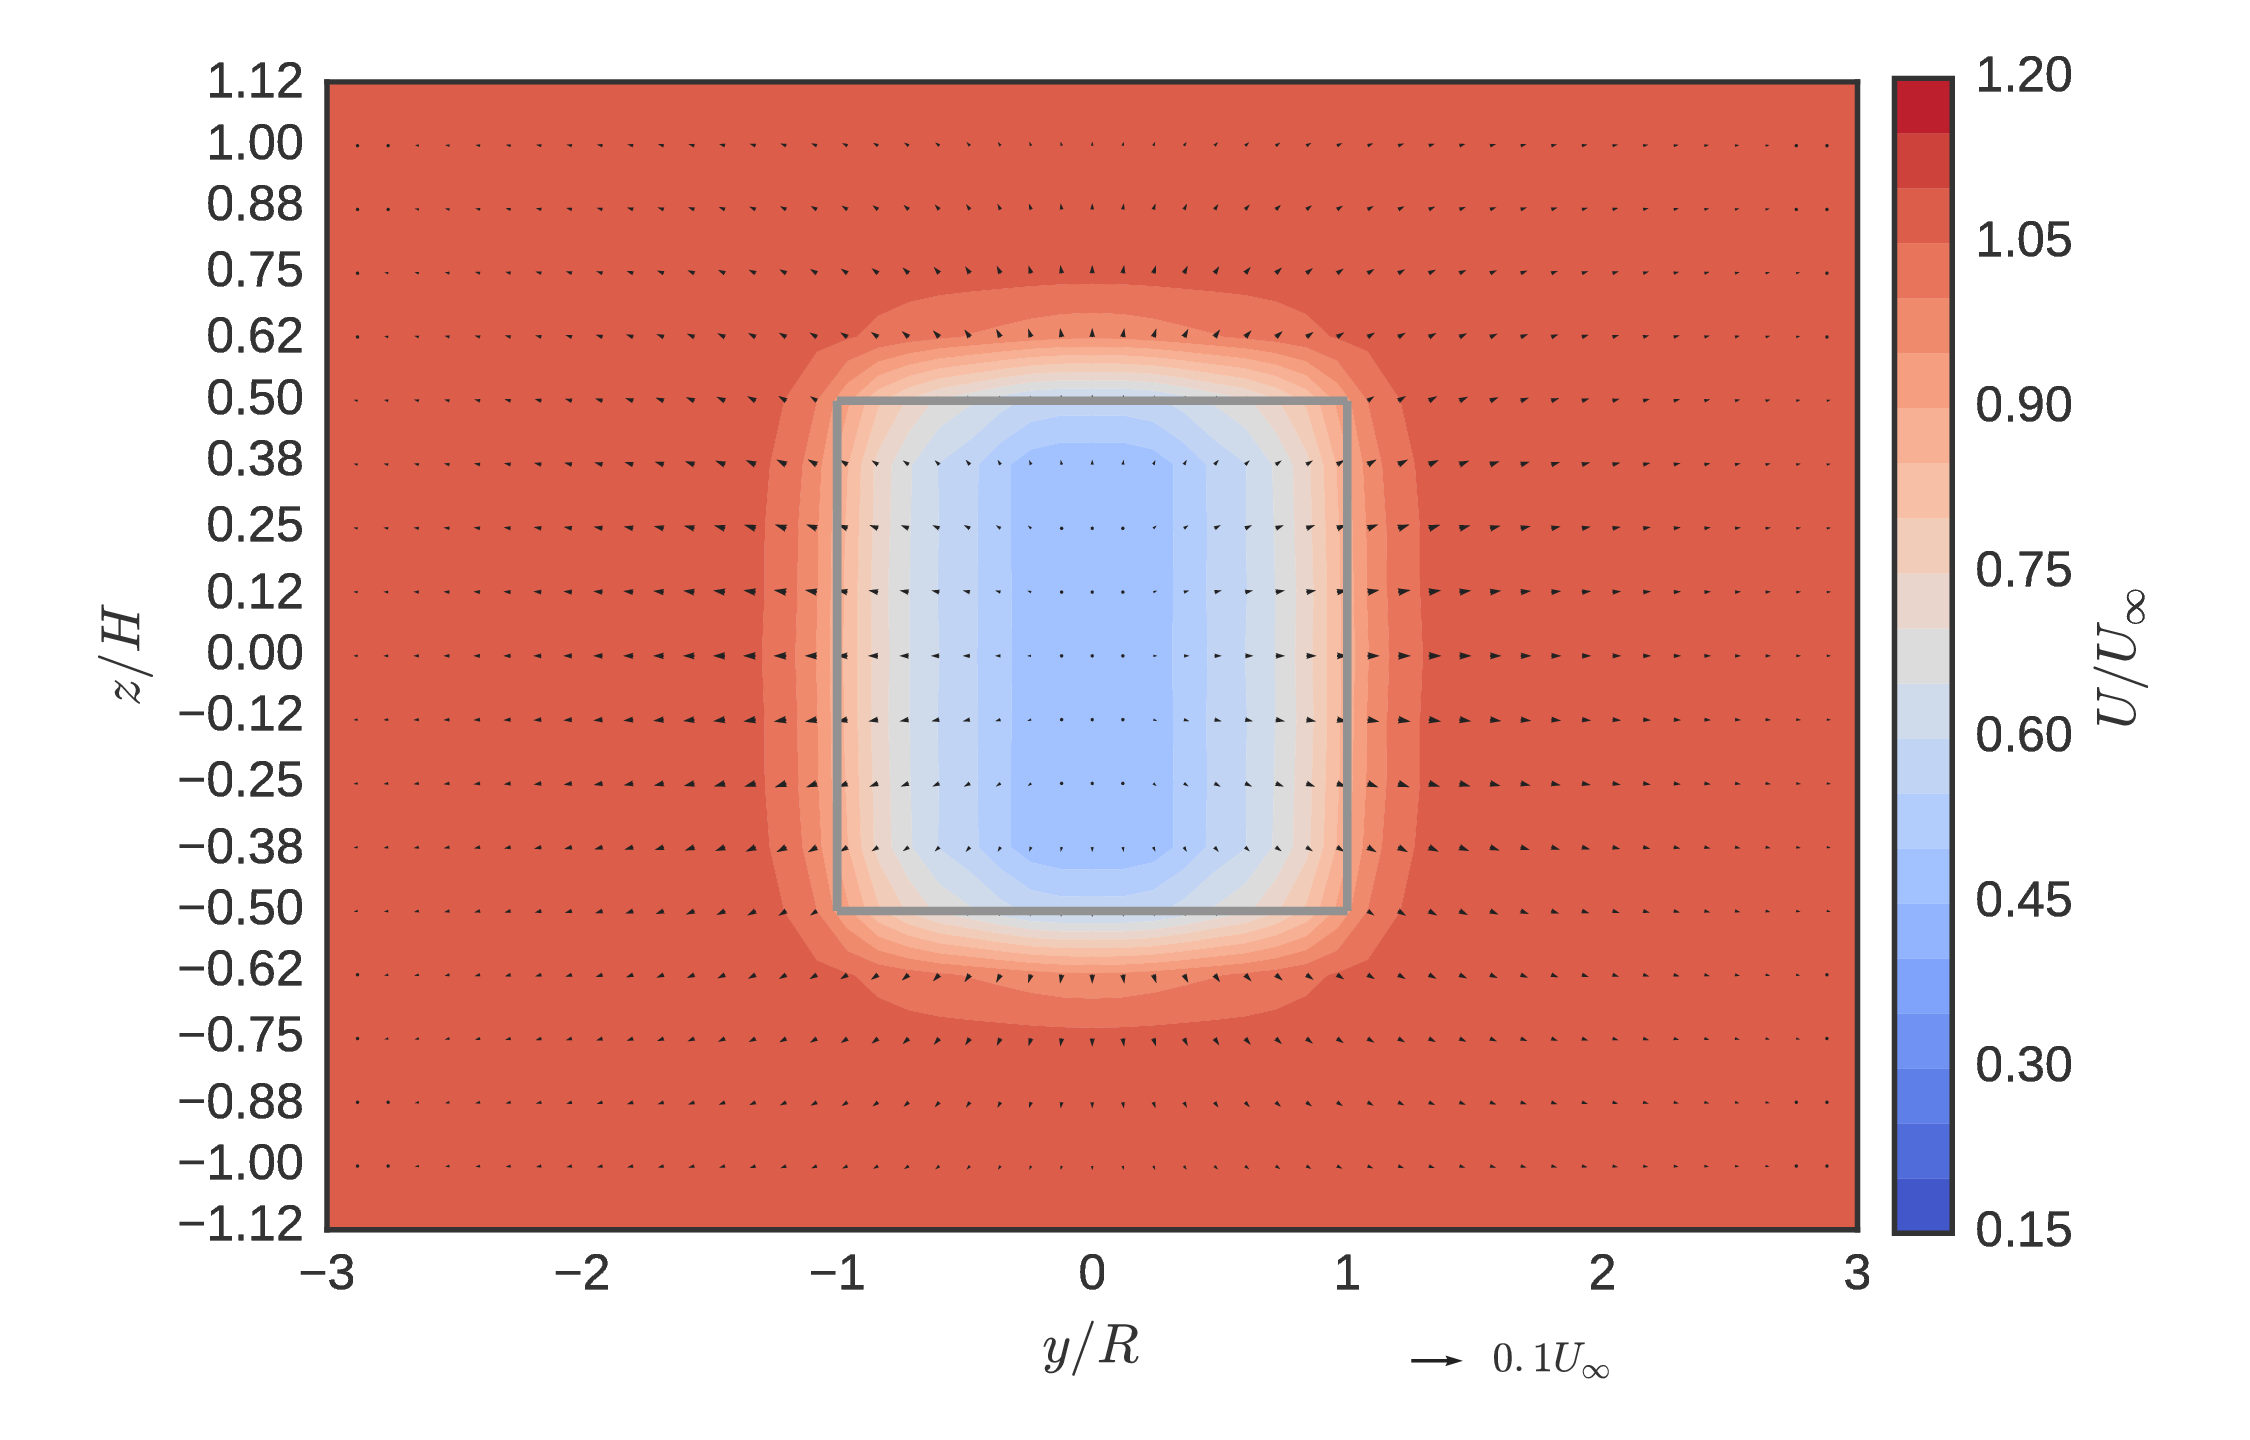
\includegraphics[clip, trim=0 0.25in 0 0.5in,
    width=0.75\textwidth]{AD_meancontquiv}

    \caption{Mean velocity predictions at $x/D=1$ from the RANS actuator disk
        numerical model. Vectors are cross-stream and vertical velocities; contours
        are streamwise velocity.}
    
    \label{fig:AD-contours}
\end{figure}

\begin{figure}
    \centering 
    
    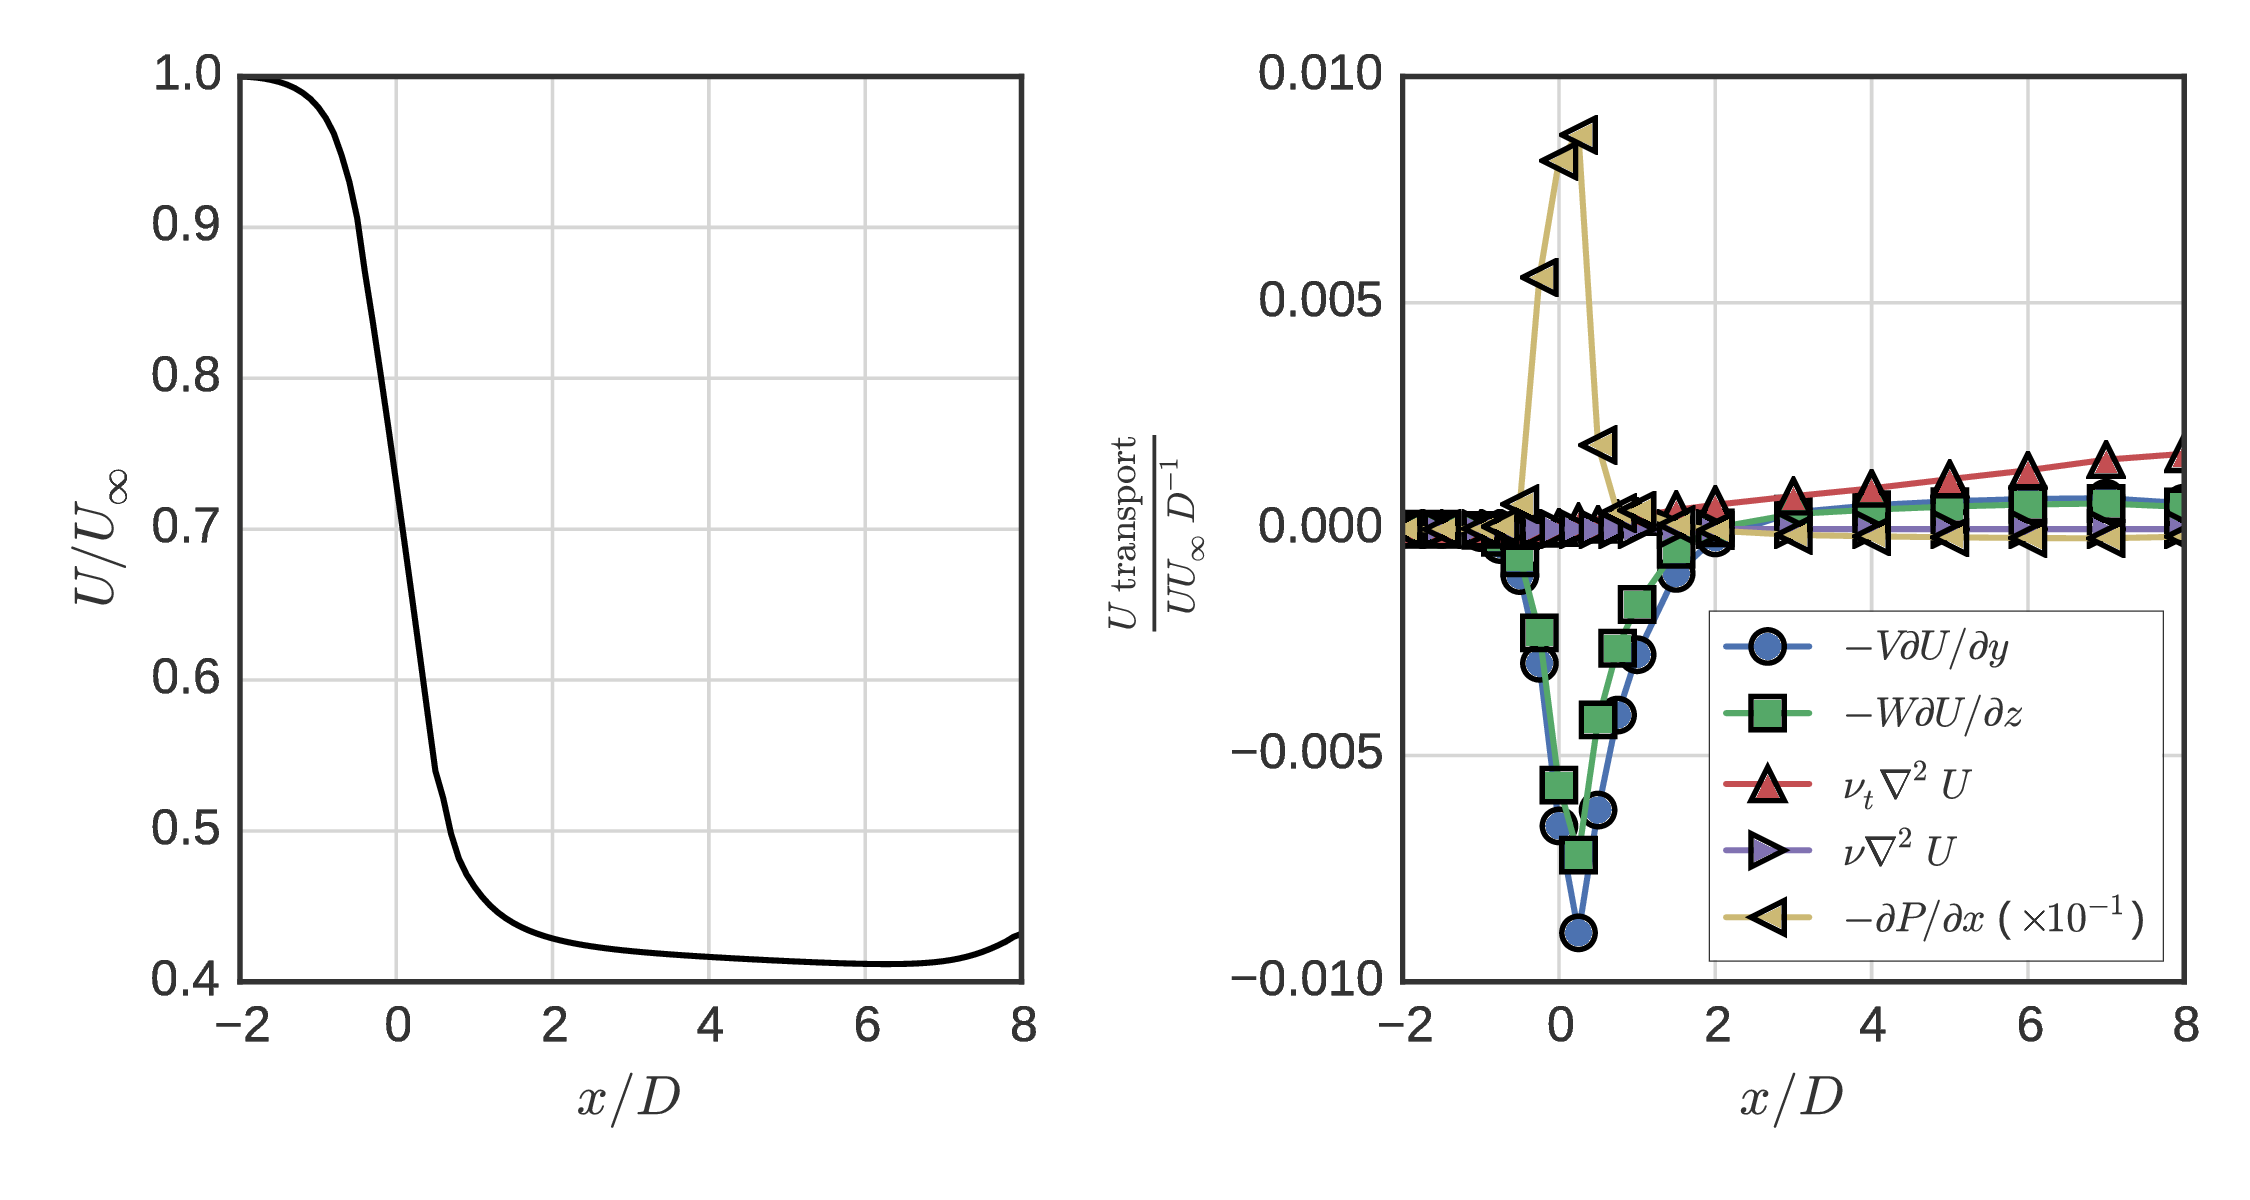
\includegraphics[width=\textwidth]{AD_streamwise}
    
    \caption{Downstream evolution of the centerline streamwise velocity (left)
        and normalized momentum transport terms (right) averaged over $y$--$z$
        slices from the actuator disk RANS simulation.} 
    
    \label{fig:AD-streamwise}
\end{figure}

\section{Conclusions}

Detailed measurements were performed in the near-wake of a vertical axis
cross-flow turbine operating at peak power coefficient. The following essential
features were identified:

\begin{enumerate}
    \item Asymmetry and three-dimensionality in the mean velocity field. 
    
    \item Mean streamwise swirling flow, or vorticity produced by blade tip and
    dynamic stall vortex shedding, which propels fluid towards the wake's center
    and makes mean vertical advection the largest contributor to streamwise
    momentum and mean kinetic energy recovery.
    
    \item Asymmetric turbulence generation due to the effects of dynamic stall
    being more pronounced on one side of the turbine.
\end{enumerate}

The most dominant timescale induced into the wake is the blade passage period. 
The $+y$ side of the turbine contains more coherent motion at this
frequency, as stalling is less prevalent there. The reduced separation due to 
stall also leads to lower magnitudes of turbulence kinetic energy on the $+y$ 
side. 

Regarding recovery of the mean streamwise momentum and kinetic energy, it was
calculated from the wake velocity measurements that vertical advection is more
than twice as large as transport by turbulent fluctuations, which may explain
why CFT wakes entrain free stream kinetic energy more effectively than their AFT
counterparts. The importance of the vertical flow created by the turbine showed
that array flow simulations will need to be carried out in three dimensions to
produce accurate results. Considering how high power coefficient estimates are
in 2-D simulations \cite{Li2013}, it logically follows that 3-D effects
significantly decrease the power output of a single turbine, but this uncaptured
power helps pull more power from outside the array. This also raises interesting
questions with respect to how cross-flow turbine blades should be
``terminated'', i.e., reducing blade tip vortices by winglets or inhibiting them
with end struts or end disks, as commonly done, may increase the performance of
individual CFTs, however, free ends that produce tip vortices may be
advantageous in an array setting to increase the wake recovery rate.

A commonly used, simple turbine forcing parameterization---an actuator
disk---was assessed for predicting the near-wake characteristics of this turbine
with a RANS simulation. The actuator disk model was found to be a poor
representation of a CFT, despite its computational efficiency and use in
research and industry. It is suggested that an actuator disk with a non-uniform
force distribution or a collection of actuator lines~\cite{Sorensen2002,
    Shamsoddin2014} may produce the asymmetry and unsteadiness that is
characteristic of the CFT near-wake and will be necessary to predict performance
of closely-spaced arrays that cross-flow turbines are thought to enable. The
actuator line method is investigated later in Chapter~\ref{chap:ALM}.
